\documentclass[english]{scrartcl}
\usepackage[T1]{fontenc}
\usepackage[latin9]{inputenc}
\usepackage{babel}
\usepackage{graphicx}
\usepackage{listings}
\usepackage{amsmath}
\usepackage{url}
% 
\renewcommand{\tt}{\normalfont \ttfamily}

\begin{document}
\title{Fitting with Adaptive Weights}
\author{R. Steven Turley}
\date{April, 2018}

\maketitle
\tableofcontents{}

\section{Introduction}

One of the difficult judgment calls required when fitting data is the
correct weighting to use for the various data points. This document
is an investigation of the results of various weighting schemes on the
fits I get for reflectance data from a thin-film mirror. I've chosen
to add noise and model errors of various kinds myself so I could study
how these variations changed my fits.

\subsection{Python}
I chose to do my analysis in python mostly for pragmatic reasons. At
the time of this writing, I am serving as a Program Officer at the
National Science Foundation. Python is available to me there, but other
choices such as Mathematica, MATLAB, and C++ are not available while
I am at NSF. Furthermore, the text-based nature of the python code allows
me to use a convenient version control system to track my changes. (That's
also one of the reasons I am using \LaTeX for this documentation. Since
the time involved in these fits isn't significant, the relative inefficiency
of untuned python code isn't an issue.

The primary purpose of this document, however, is to investigate issues
which should be pretty language agnostic. I'll include some python
examples to illustrate points (mostly in the appendix), but the complete documentation of the code is found elsewhere \cite{rst18}.

\subsection{Model Mirror}
My initial model mirror for these investigations has the parameters shown
in Table~\ref{tab:model-mirror}.
\begin{table}[htb]
\begin{center}
\begin{tabular}{| c | c |}\hline
material&thickness (nm)\\ \hline\hline
vacuum & 0 \\
AlF$_3$&18\\
Al&50\\
SiO$_2$&1.6\\
Si&0\\ \hline
\end{tabular}
\end{center}
\caption{\label{tab:model-mirror}Model mirror used for calculations.}
\end{table}
The calculations were done at a wavelength of $\lambda=12\,\mbox{nm}$ for
160 points between 0.5 and 80 degrees. For this ideal mirror, I assumed
no roughness. The reflectance as a function of angle is shown in
Figure~\ref{fig:model}
\begin{figure}[htb]
  \begin{center}
    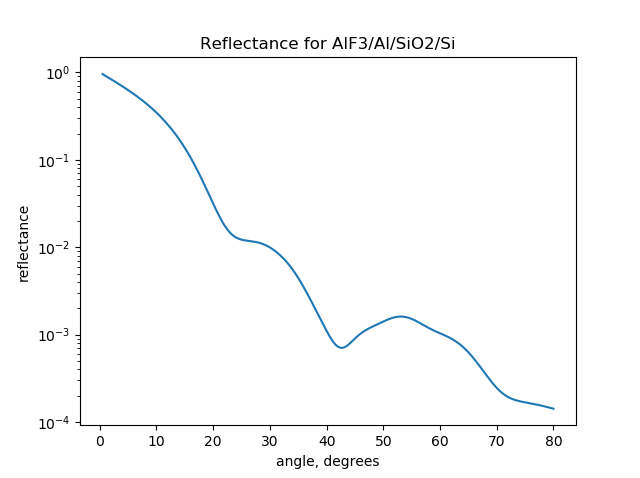
\includegraphics[width=0.75\textwidth]{images/model}
  \end{center}
  \caption{\label{fig:model}Reflectance from model mirror with the
  composition from Table~\ref{tab:model-mirror}.}
\end{figure}
The reflectance has the following characteristics which are important
in effective fitting:
\begin{itemize}
\item varies by orders of magnitude of the range of angles chosen
\item has minima characteristic of layer thicknesses
\item minima are a result of interference from more than one interface
\end{itemize}

For reference purposes, the python code used to compute reflectance
with the Parratt formula is given in Appendix~\ref{sec:Parratt-py}.

\section{Model Error}
\subsection{Statistical Uncertainty}
For the purposes of this study, I have assumed the measurements have
two error contributions. The first is instrumentation uncertainty
proportional to the signal. The second is a base noise level independent
of the signal. Let $\eta(\sigma)$ be a normally distributed random number
with mean $0$ and rms width $\sigma$. If the exact reflectance is
$r(\theta)$, then the measured reflectance would be
\begin{equation}
f(\theta)=r(\theta)[1+\eta(\sigma_p)]+\eta(\sigma_c)\;.
\end{equation}
This was implemented in Python using the numpy library (imported as np).
The numpy array rfl holds the exact reflectance at angles stored in
the numpy array thr.
\begin{lstlisting}
sigmap = 0.05 # proportiional noise
sigmac = 1e-4 # constant noise
refn = (rfl*(1+sigmap*np.random.randn(np.size(thr)))+
        sigmac*np.random.randn(np.size(thr)))
\end{lstlisting}
As you'll note in the code, I used $\sigma_p=0.05$ and $\sigma_c=10^{-4}$.

The actual error is more complicated than this. For instance, the
reflectance is a ratio of $I$, the reflected signal, to $I_0$, the signal
passing straight through to the detector. The $I$ measurements were taken
with more than one gain, each of which had different dark currents (with
different values of $\sigma_c$. Additional errors should be added in
quadrature for $I_0$. The analog to digital converter (ADC) introduced
digitization noise, which would need to be accounted for as well.

Nevertheless, there is evidence that the model I've used accounts for
the most significant qualitative features of the expected statistical
uncertainty.

Figure~\ref{fig:noise}
\begin{figure}[htb]
  \begin{center}
    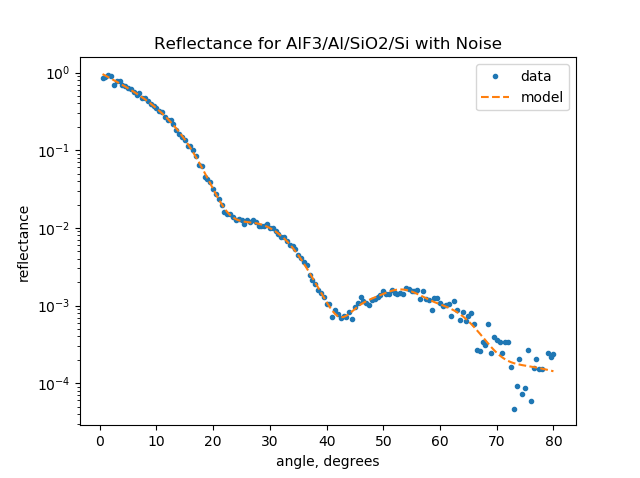
\includegraphics[width=0.75\textwidth]{images/noise}
  \end{center}
  \caption{\label{fig:noise}Reflectance from model mirror with random
  noise added}
\end{figure}
is a graph of the exact data and the data with
random noise added as above. Note that the noise is biggest at high
angles where the small reflectance makes the contribution from the
constant part of the error most significant. Also note that the noise
looks unsymmetrically distributed on a semilog plot as shown here.
That is because equal values of error in the positive and negative
directions have unequal weights on a logarithmic scale.

\subsection{Systematic Error}\label{sec-syserr}
Our models for the reflectance undoubtedly are imperfect. As implemented,
they don't correctly account for variations in layer thickness, interfacial
roughness, and incorrect assumptions about material thicknesses and
optical constants. I will study these effects as well by purposely adding
this kind of error in later models.

The example I have used for systematic error in this case was omitting the
SiO$_2$ layer between the Si substrate and the Al. This gives the same
kind of fitting challenge I often see in fitting real data: a good fit
for low angles and a degraded fit for higher angles.
Figure~\ref{fig:with-and-without} is a plot of the two exact reflectances
for this case.
\begin{figure}[htb]
	\begin{center}
		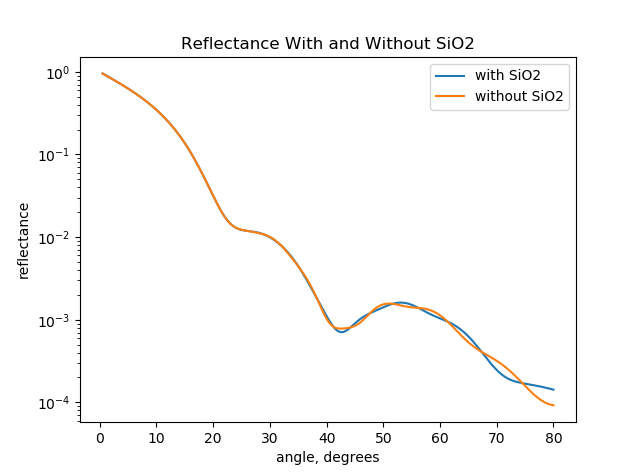
\includegraphics[width=0.75\textwidth]{images/with-and-without}
	\end{center}
	\caption{\label{fig:with-and-without}Reflectance from model mirror with and
		without the SiO$_2$ layer}
\end{figure}


\section{Fits}
The process of weighted least squares fitting involves minimizing
the function
\begin{equation}
\chi^2 = \sum_i\left[\frac{y_i - r(\theta_i;
	\vec{b})}{\sigma_i}\right]^2\label{eq:chisq}
\end{equation}
where $y_i$ are the measured data points at the measurement angles
$\theta_i$ and $\sigma_i$ are the uncertainties at those points. The
function $r$ is the computed reflectance which depends both on the angle
$\theta_i$ and the fit parameters $\vec{b}$. For the purposes of
the present exercise, I chose to fit the index of refraction of
the top AlF$_3$ layer and the thickness of that layer.
\subsection{Unweighted Fit}
I first fit the data using equal weights for each point. In other words,
I minimized Equation~\ref{eq:chisq} with $\sigma+_i=1$. Here are the
important parts of the python code for doing the fit.
\begin{lstlisting}
AlIndex = Index("Al")
SiIndex = Index("Si")
SiO2Index = Index("SiO2")
AlF3Index = Index("AlF3")

wl = 12
alndx = AlIndex.at(wl)
sindx = SiIndex.at(wl)
sio2ndx = SiO2Index.at(wl)
alf3ndx = AlF3Index.at(wl)

n=np.array([1+0j, alf3ndx, alndx, sio2ndx, sindx])
t=np.array([0, 18, 50, 1.6, 0])
thr = np.linspace(0.5,80,160)
p0 = np.array([alf3ndx.real, alf3ndx.imag, 18])
def f(thr, n, k, t):
    ndx = np.array([1+0j, n+k*1j, alndx, sio2ndx, sindx])
    th = np.array([0, t, 50, 1.6, 0])
    return [Parratt(ndx ,th, thetad, wl) for thetad in thr]
sigma = np.ones(np.size(thr))
popt, pcov = curve_fit(f, thr, refn, p0, sigma,
    absolute_sigma=False)

\end{lstlisting}
The python code uses the Index class listed in Appendix~{sec:Index}
to read the index of refraction data from the reference files on volta
and interpolate to the desired wavelength. The function \verb+f+
computes the reflectance given the fit parameters n, k, and t which are
passed to it. The fit is done using the scipy.optimize routine
curve\_fit. That routine returns the optimal fit parameters in the
array popt and the covariance matrix as pcov.

For this fit I got the values shown in Table~\ref{tab:unweighted}.
\begin{table}[htb]
\begin{center}
\begin{tabular}{| c | c | c |}
\hline
quantity & exact & fit\\ \hline\hline
n & $0.9717$ & $0.9718\pm 0.00078$\\
k & $0.0249$ & $0.0238\pm 0.0017$\\
thickness & $18.0$ & $18.25\pm 1.82$\\ \hline
\end{tabular}
\end{center}
\caption{\label{tab:unweighted}Results from an unweighted fit}
\end{table}
Note that the relative  uncertainty of the thickness is much larger than
the uncertainty of the index of refraction. This is because of unweighted
fit emphasizes agreement with the data most heavily at low angles. The
reflectance at these angles depends more on $n$ and $k$ than on the
thickness.
Figure~\ref{fig:unweighted}
\begin{figure}[htb]
  \begin{center}
    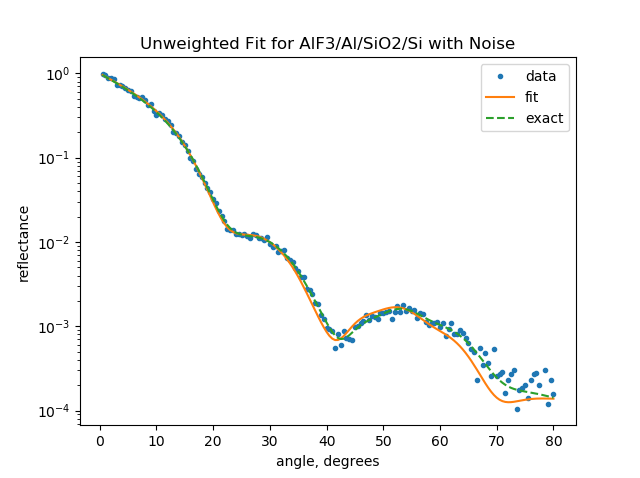
\includegraphics[width=0.75\textwidth]{images/eqweight}
  \end{center}
  \caption{\label{fig:unweighted}Fit of reflectance from model mirror with random noise added using $\sigma_i=1$.}
\end{figure}
is a plot of the data, fit, and exact reflectance with no noise. Note
that the fit is most significantly different form the exact answer
at the highest angles where the reflectance is smallest.

\subsection{Proportionally Weighted Fit}
I redid the fit using a value of $\sigma_i$ equal to the product
of $\sigma_p$ and the model reflectance. Here is the python code
for that change.
\begin{lstlisting}
sigma=sigmap*np.array(rfl)
popt, pcov = curve_fit(f, thr, refn, p0, sigma,
      absolute_sigma=True)

\end{lstlisting}
The values of $\sigma_i$ are mostly reasonable estimates of the
absolute error in the this case, so I set \verb+absolute_sigma=True+.
Table~\ref{tab:propweight} give thje values for the fitted parameters
in this case.
\begin{table}[htb]
\begin{center}
\begin{tabular}{| c | c | c |}
\hline
quantity & exact & fit\\ \hline\hline
n & $0.9717$ & $0.9719\pm 0.00011$\\
k & $0.0249$ & $0.0251\pm 0.00012$\\
thickness & $18.0$ & $17.933\pm 0.013$\\ \hline
\end{tabular}
\end{center}
\caption{\label{tab:propweight}Results from an fit with a
proportional weight $\sigma_i = \sigma_p r(\theta_i)$}
\end{table}
Note the improvement of the uncertainties in the fit for all of the
parameters, but especially the thickness. Part of the overall reduction
in uncertainties is that more points are contributing significantly
to the sum in Equation~\ref{eq:chisq}. The reason the thickness is
so much better is because of the extra importance put on the high
angle points.  Figure~\ref{fig:propweight} is a graph of the data, fit,
and exact reflectance for this case.
\begin{figure}[htb]
  \begin{center}
    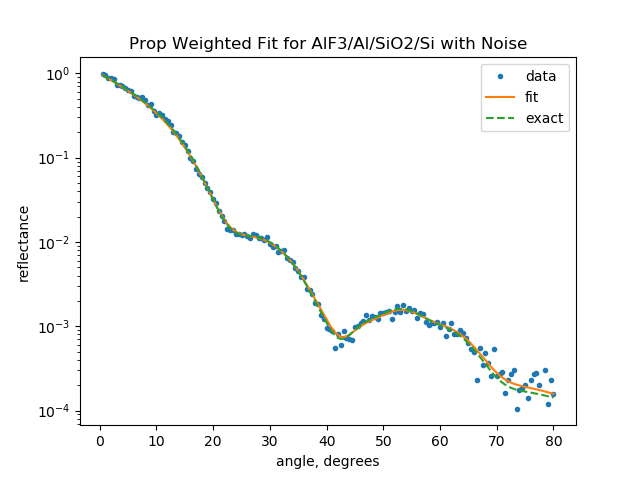
\includegraphics[width=0.75\textwidth]{images/propweight}
  \end{center}
  \caption{\label{fig:propweight}Fit of reflectance from model mirror with random noise added using a weight proportional to the reflectance, $\sigma_i=\sigma_p r(\theta_i)$.}
\end{figure}

\subsection{Combined Weights}
The most logical weights to use for the fits would be
\begin{equation}
\sigma_i = \sqrt{[\sigma_p r(\theta_i)]^2+\sigma_c^2}\label{eq:combined}
\end{equation}
since this corresponds exactly to our error model. Here is
the relevant python code.
\begin{lstlisting}
sigma = np.sqrt((sigmap*np.array(rfl))**2+sigmac**2)
\end{lstlisting}
The fit
for the proportional weights shown in Figure~\ref{fig:propweight}
was already so good, there isn't much difference you can see in the
graphical residuals. However, there are some interesting differences
in the fit parameters listed in Table~\ref{tab:combweight}.
\begin{table}[htb]
\begin{center}
\begin{tabular}{| c | c | c |}
\hline
quantity & exact & fit\\ \hline\hline
n & $0.9717$ & $0.9717\pm 0.00014$\\
k & $0.0249$ & $0.0248\pm 0.00025$\\
thickness & $18.0$ & $18.0005\pm 0.0310$\\ \hline
\end{tabular}
\end{center}
\caption{\label{tab:combweight}Results from an weighted fit with a
combined uncertainty given by Equation~\ref{eq:combined}.}
\end{table}
The uncertainties are higher, but probably more accurate and the
fit parameters are better.

\subsection{Systematic Errors}
Systematic errors arise when the model of our mirror
doesn't match the actual mirror for some reason. This would
be due to missing layers, incorrect assumptions about layer
thicknesses, incorrect assumptions about the index of
refraction, or a gradient in the layer thickness. In this
section, I'll address how systematic errors affect our
fits and the appropriate weights to use when fitting them.

I will use the model introduced in Section~\ref{sec:syserr},
where a sample with a SiO$_2$ layer is modeled without
including that layer.

\subsubsection{Constant Weights}
The fit using constant weights is better than I expected
a first blush. Because the constant weights put most
of their emphasis on the region where the model and data
agree (at low angles) the fit is actually quite good.
Table~\ref{tab:mconst} shows the results of this fit.
\begin{table}[htb]
	\begin{center}
		\begin{tabular}{| c | c | c |}
			\hline
			quantity & exact & fit\\ \hline\hline
			n & $0.9717$ & $0.9717\pm 0.00000$\\
			k & $0.0249$ & $0.0249\pm 0.00001$\\
			thickness & $18.0$ & $17.9999\pm 0.00729$\\ \hline
		\end{tabular}
	\end{center}
	\caption{\label{tab:mconst}Results from an unweighted fit with a bad model}
\end{table}
The data and fit are shown in Figure~\ref{fig:mconst}.
\begin{figure}[htb]
	\begin{center}
		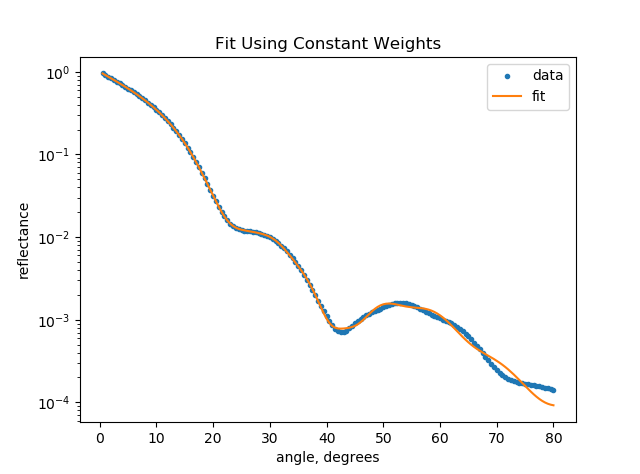
\includegraphics[width=0.75\textwidth]{images/mconst}
	\end{center}
	\caption{\label{fig:mconst}Fit of reflectance from model mirror using an incomplete model and constant weights}
\end{figure}

\subsubsection{Proportional Weights}
Using proportional weights, the fit is worse, but is a more
accurate result of using the incorrect model. The fits
were done with absolute\_sigma=True. Using
absolute\_sigma=False
gives larger uncertainties in the fit parameters by about
a factor of two.
Table~\ref{tab:mprop} shows the results of the fit
in this case.
\begin{table}[htb]
	\begin{center}
		\begin{tabular}{| c | c | c |}
			\hline
			quantity & exact & fit\\ \hline\hline
			n & $0.9717$ & $0.9720\pm 0.00011$\\
			k & $0.0249$ & $0.0257\pm 0.00013$\\
			thickness & $18.0$ & $18.0886\pm 0.01231$\\ \hline
		\end{tabular}
	\end{center}
	\caption{\label{tab:mprop}Results from a proportionally
		weighted fit with a bad model}
\end{table}
Note that even thought the fit is "worse," the uncertainties
computed using statistical considerations are a reasonable
estimate of the amount they are off.
Figure~\ref{fig:mconst} shows the exact data and the fit.
\begin{figure}[htb]
	\begin{center}
		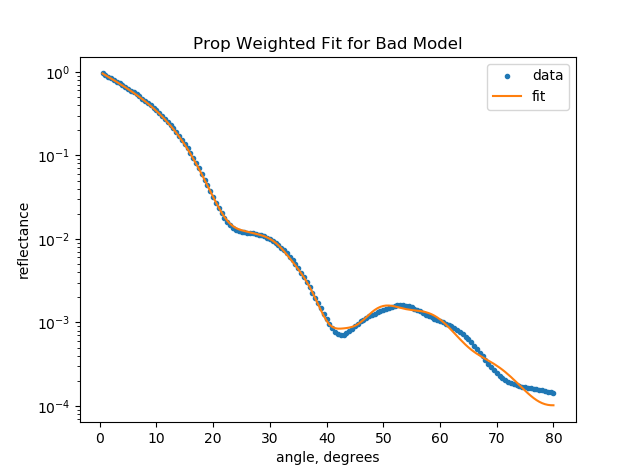
\includegraphics[width=0.75\textwidth]{images/mprop}
	\end{center}
	\caption{\label{fig:mprop}Fit of reflectance from model mirror using an incomplete model and proportional weights}
\end{figure}

\section{Weight Selection}
Given how critical it is to get the weights correct in
fitting, it is important to know what the signatures are
of incorrect weights and how these might be determined
empirically.
\subsection{Statistical Errors Only}
If the only contribution to the errors is statistical,
the relative size of the weighted residuals is a good
clue. On average, the residuals should have the same
magnitude across the range of angles.

As an illustration, Figure~\ref{fig:res-equalweight}
is a graph of the weighted residuals
\begin{equation}
r=\frac{f(x_i)-y_i}{\sigma_i}
\end{equation}
for a fit with constant weights.Note how the weighted
residuals are larger for low angles where the reflectance
is higher than for higher angles where the reflectance
is lower.
\begin{figure}[htb]
  \begin{center}
    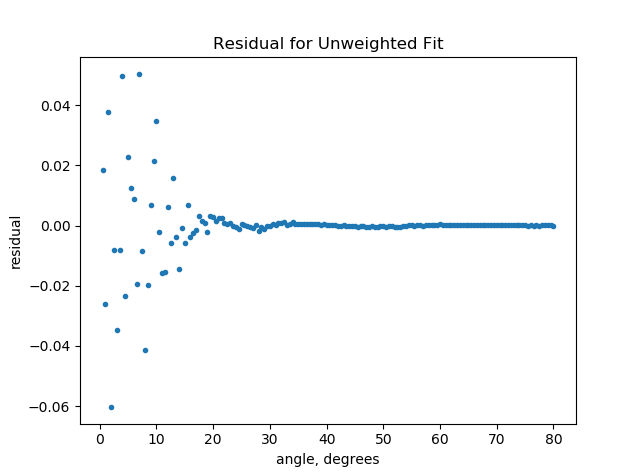
\includegraphics[width=0.75\textwidth]{images/res-equalweight}
  \end{center}
  \caption{\label{fig:res-equalweight}Weighted residuals
  from a fit with equal weights}
\end{figure}

Figure~\ref{fig:res-propweight} is the same plot for a fit
using proportional weights.
\begin{figure}[htb]
  \begin{center}
    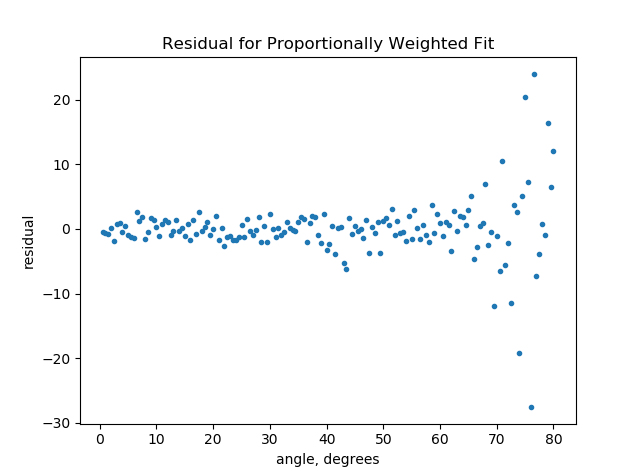
\includegraphics[width=0.75\textwidth]{images/res-propweight}
  \end{center}
  \caption{\label{fig:res-propweight}Weighted residuals
  for a fit with proportional weights}
\end{figure}
Note how the largest weighted residuals are on the high
angle side of the graph where the constant error term
is significant and hasn't been correctly added.

Figure~\ref{fig:res-combweight} is the same plot for a fit
using the combined weight from Equation~\ref{eq:combined}.
\begin{figure}[htb]
  \begin{center}
    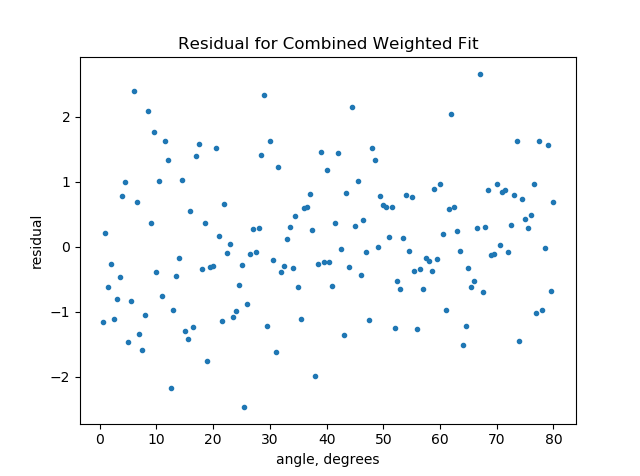
\includegraphics[width=0.75\textwidth]{images/res-combweight}
  \end{center}
  \caption{\label{fig:res-combweight}Weighted residuals
  for a fit with combined weights from Equation~\ref{eq:combined}}
\end{figure}
Note that the errors all have equal average
magnitudes and an
rms size of about 1. This is what an ideal plot of weighted
residuals would look like if the error is only statistical.

\subsection{Systematic Errors}
It is more subtle to find the correct weighting when
the errors are systematic rather than statistical. The
signature of systematic errors is having the weighted
residuals characteristically on one side or the other
of zero, rather than being randomly distributed as
in Figure~\ref{fig:res-combweight}. Also, it may or
may not be reasonable to expect $chi^2$ to equal the
number of data points in this case. Figure~\ref{fig:mrp} is
a plot of the normalized residuals in this case.
\begin{figure}[htb]
	\begin{center}
		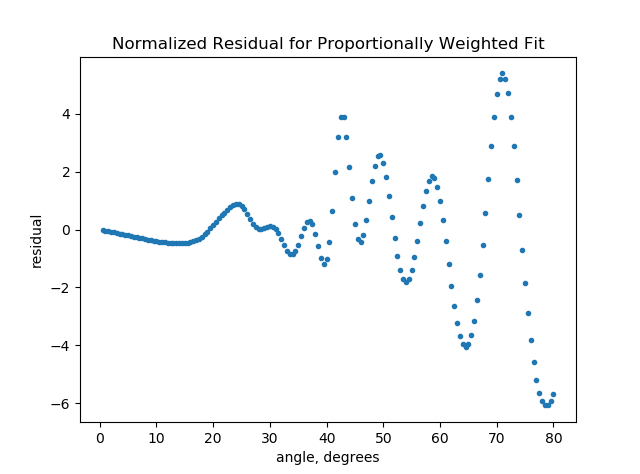
\includegraphics[width=0.75\textwidth]{images/mrp}
	\end{center}
	\caption{\label{fig:mrp}Normalized residual from
	fitting the mirror with a model error and proportional
	weights}
\end{figure}

\subsection{Combined Errors}
Of course, in practice, we can anticipate a combination
of statistical and systematic errors.

\appendix

\section{Parratt Function\label{sec:Parratt-py}}
This is the python code used to compute reflectance from a thin-film
mirror.
\begin{lstlisting}
def Parratt(n, x, thetad, lam, fractions=0, sigma=0):
    """Reflectance from a multilayer mirror
    
    Parameters
    ----------
    n : np.array of index of refractions for stack starting with 
        index of the incident layer
    n2 : number
        index of the other layer
    thetad : number
        incident angle in degrees
    lam : number
        wavelength in nanometers
    fractions : number
        fraction of light with s polarization. If zero, this is
        calculated using Gullikson formula for synchrotron
    sigma : array of number
        interface roughness in nm
        
    Returns
    -------
    ref: number
        reflectance of the layer for s polarization
        
    Example
    -------
    >>> lam = 15
    >>> AlIndex = refl.Index('Al')
    >>> alndx = AlIndex.at(lam)
    >>> SiO2Index = refl.index('SiO2')
    >>> sio2ndx = SiO2Index.at(lam)
    >>> n = np.array([1, alndx, sio2ndx])
    >>> t = np.array([0, 20, 0])
    >>> thetad = 20
    >>> Parratt(n, t, thetad, lam)
    0.012606490280013215
    """
    if fractions==0:
        fractions = fracs(lam)
    fractionp = 1-fractions
    S = np.sqrt(n**2-np.cos(thetad*np.pi/180)**2)
    k = 2*np.pi/lam
    C = np.exp(2j*S*x*k)
    rs = 0
    rp = 0
    
    qz = k*np.sin(thetad*np.pi/180) # for DW correction
    if sigma == 0:
        sigma = np.zeros(n.size-1)
    eta = np.exp(-2*qz**2*sigma**2) # DW roughness correction
    
    for m in range(n.size-1, 0,-1):
        fs = (S[m-1]-S[m])/(S[m-1]+S[m])
        fp = ((n[m]**2 * S[m-1] - n[m-1]**2 * S[m])/
              (n[m]**2 * S[m-1] + n[m-1]**2 * S[m]))
        rs = C[m-1]*(fs*eta[m-1]+rs*eta[m-1]**2)/(
              1+fs*rs*eta[m-1])
        rp = C[m-1]*(fp*eta[m-1]+rp*eta[m-1]**2)/(
              1+fp*rp*eta[m-1])
    return fractionp*np.abs(rp)**2+fractions*np.abs(rs)**2
     
\end{lstlisting}

\section{Index Class\label{sec:Index}}
Here is a listing of the python code used to read and interpolate
index of refraction data from the volta reference files.
\begin{lstlisting}
import pandas
from scipy.interpolate import interp1d

class Index:
    """ Index of refraction from volta
    
    Constructor Parameters
    ----------------------
    material : string
        material from base of .nk file on volta
    
    Method
    ------
    at(wavelength) : returns interpolated index at the given
        wavelength in nm. Wavelength can by an np.array
    
    Example
    -------
    alndx=Index('Al')
    lam=np.linspace(10,400,200)
    ndx=alndx.at(lam)
    """
    def __init__(self, material):
        df=pandas.read_table(
              "http://volta.byu.edu/nk/"+material+".nk",
              comment=';',delim_whitespace=True)
        val=df.values
        lam=val[:,0]/10
        ndx=val[:,1]+val[:,2]*1j
        self.at=interp1d(lam,ndx,'cubic')

\end{lstlisting}

\begin{thebibliography}{9}
\bibitem{rst18}
R. Steven Turley, ``Calculating and Fitting Thin-Film Mirror
Reflectance with Python,'' BYU Scholar's Archive, 2018.
\end{thebibliography}
\end{document}